\documentclass{beamer}
\usepackage{graphicx}
\usepackage{verbatim}
\usepackage{amsmath}
\usepackage{amsfonts}
\usepackage{setspace}
% \usepackage{beamerthemesplit} // Activate for custom appearance

\title{Regression Introduction and Estimation Review}
\author{Dr. Frank Wood}

\date{}

\DeclareMathOperator*{\Ave}{\mathbb{E}}
\DeclareMathOperator*{\Var}{Var}

\begin{document}

\frame{\titlepage}

\frame[t] {%%% change pic %%%
 \frametitle{Quick Example - Scatter Plot}
\begin{figure}
  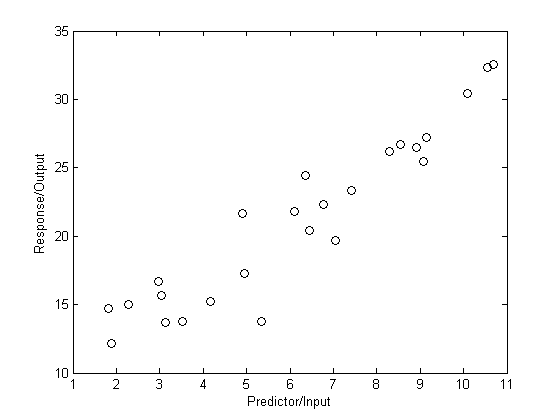
\includegraphics[height=60mm]{qeg.png}
\end{figure}
}

\frame[t] {
 \frametitle{Linear Regression}
\begin{itemize}
\item Want to find parameters for a function of the form
$$Y_i = \beta_0 + \beta_1 X_i + \epsilon_i$$
\item Distribution of error random variable not specified
\end{itemize}
}

\frame[t] { %%% change pic %%%
 \frametitle{Quick Example - Scatter Plot}
\begin{figure}
  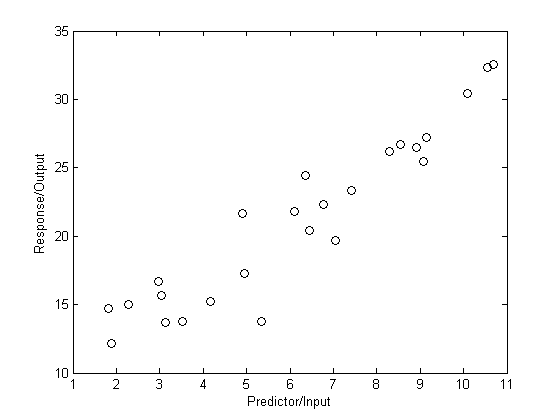
\includegraphics[height=60mm]{qeg2.png}
\end{figure}
}

\frame[t] {
 \frametitle{Formal Statement of Model}
$$Y_i = \beta_0 + \beta_1 X_i + \epsilon_i$$
\begin{itemize}
\item $Y_i$ value of the response variable in the $i^{th}$ trial
\item $\beta_0$ and $\beta_1$ are parameters
\item $X_i$ is a known constant, the value of the predictor variable in the $i^{th}$ trial
\item $\epsilon_i$ is a random error term with mean $\Ave(\epsilon_i)$ and variance
$\Var(\epsilon_i)=\sigma^2 $
\item $i = 1,\ldots,n$
\end{itemize}
}

\frame[t] {
 \frametitle{Properties}
\begin{itemize}
\item The response $Y_i$ is the sum of two components
\begin{itemize}
\item Constant term $\beta_0 + \beta_1 X_i$
\item Random term $\epsilon_i$
\end{itemize}
\item The expected response is
\begin{eqnarray*}
\Ave(Y_i) &=& \Ave(\beta_0 + \beta_1 X_i + \epsilon_i)\\
 &=& \beta_0 + \beta_1 X_i + \Ave(\epsilon_i)\\
&=& \beta_0 + \beta_1 X_i
\end{eqnarray*}
\end{itemize}
}

\frame[t] {
 \frametitle{Expectation Review}
\begin{itemize}
\item Definition
$$\Ave(X) = \Ave(X) = \int X P(X) dX, \, X \in \mathcal{R}$$
\item Linearity property \begin{eqnarray*}
\Ave(aX) &=& a \Ave(X)\\
\Ave(aX + bY) &=& a\Ave(X) + b\Ave(Y)
\end{eqnarray*}

\item Obvious from definition
\end{itemize}
}

\frame[t] {
 \frametitle{Example Expectation Derivation}
$$P(X) = 2X, 0 \leq X \leq 1$$
Expectation
\begin{eqnarray*}
\Ave(X) &=& \int_0^1 X P(X) dX\\
 &=& \int_0^1 2X^3 dX\\
&=& \frac{2X^2}{3} |_0^1\\
&=& \frac{2}{3}
\end{eqnarray*}

}

\frame[t] {
 \frametitle{Expectation of a Product of Random Variables}
If X,Y are random variables with joint distribution $P(X,Y)$ then
the expectation of the product is given by
$$\Ave(XY)=\int_{XY}XYP(X,Y)dXdY.$$
}

\frame[t] {
 \frametitle{Expectation of a product of random variables}
What if X and Y are independent? If X and Y are independent with
density functions f and g respectively then
\begin{eqnarray*}
\Ave(XY)&=& \int_{XY}XYf(X)g(Y)dXdY\\
&&= \int_X\int_Y XYf(X)g(Y)dXdY\\
&&= \int_X Xf(X)[\int_Y Yg(Y)dY]dX\\
&&= \int_X Xf(X)\Ave(Y)dX\\
&&=\Ave(X)\Ave(Y)
\end{eqnarray*}
}

\frame[t] {
 \frametitle{Regression Function}
\begin{itemize}
\item The response $Y_i$ comes from a probability distribution with mean
\begin{eqnarray*}
\Ave(Y_i) &=& \beta_0 + \beta_1 X_i
\end{eqnarray*}
\item This means the regression function is
\begin{eqnarray*}
\Ave(Y) &=& \beta_0 + \beta_1 X
\end{eqnarray*}
Since the regression function relates the means of the probability
distributions of Y for a given X to the level of X

\end{itemize}
}

\frame[t] {
 \frametitle{Error Terms}
\begin{itemize}
\item The response $Y_i$ in the $i^{th}$ trial exceeds or falls short of the value of the regression function by the error term
amount $\epsilon_i$
\item The error terms $\epsilon_i$ are assumed to have constant variance $\sigma^2$

\end{itemize}
}

\frame[t] {
 \frametitle{Response Variance}
Responses $Y_i$ have the same constant variance
\begin{eqnarray*}
\Var(Y_i) &=& \Var(\beta_0 + \beta_1 X_i + \epsilon_i)\\
 &=& \Var(\epsilon_i)\\
&=& \sigma^2
\end{eqnarray*}

}

\frame[t] {
 \frametitle{Variance ($2^{nd}$ central moment) Review}
\begin{itemize}
\item Continuous distribution $$\Var(X) = \Ave(( X -  \Ave(X) ) ^ 2) = \int (X - \Ave(X))^2 P(X) dX, \, X \in \mathcal{R}$$
\item Discrete distribution $$\Var(X) = \Ave(( X -  \Ave(X) ) ^ 2) = \sum_i (X_i - \Ave(X))^2 P(X_i), \, X \in \mathcal{Z}$$
\end{itemize}
}

\frame[t] {
 \frametitle{Alternative Form for Variance}
\begin{eqnarray*}
\Var(X) &=&\Ave( ( X -  \Ave(X) ) ^ 2 ) \\
& = &\Ave( ( X ^ 2 - 2X\Ave(X) + \Ave(X) ^ 2) ) \\
&=&\Ave( X ^ 2) - 2\Ave(X)\Ave(X) + \Ave(X)  ^ 2 \\
& =&\Ave( X ^ 2) - 2\Ave(X) ^ 2 + \Ave(X) ^ 2 \\
&=&\Ave ( X ^ 2) - \Ave(X) ^ 2.
\end{eqnarray*}

}

\frame[t] {
 \frametitle{Example Variance Derivation}
$$P(X) = 2X, 0 \leq X \leq 1$$
\begin{eqnarray*}
\Var(X) &=& \Ave((X-\Ave(X))^2) = \Ave(X^2) - \Ave(X)^2 \\
 &=& \int_0^1 2X X^2 dX - (\frac{2}{3})^2\\
&=& \frac{2X^4}{4}|_0^1- \frac{4}{9} \\
&=& \frac{1}{2} -  \frac{4}{9} =  \frac{1}{18}
\end{eqnarray*}

}

\frame[t] {
 \frametitle{Variance Properties}
\begin{eqnarray*}
\Var(aX) &=& a^2 \Var(X)\\
\Var(aX + bY) &=& a^2\Var(X) + b^2\Var(Y)\, \mathrm{if} X \perp Y \\
\Var(a +cX)  &=& c^2 \Var(X)\; \mathrm{if} a, c\; \mathrm{both\ constant}
\end{eqnarray*}
More generally
\begin{eqnarray*}
\Var(\sum a_i X_i) &=& \sum_i\sum_j a_i a_j \mathrm{Cov}(X_i,X_j)
\end{eqnarray*}

}

\frame[t] {
 \frametitle{Covariance}
\begin{itemize}
\item The covariance between two real-valued random variables X and Y, with expected values $\Ave(X) = \mu$ and $\Ave(Y) = \nu$ is defined as
$$Cov(X,Y)=\Ave((X-\mu)(Y-\nu))$$
\item Which can be rewritten as\begin{eqnarray*}
Cov(X,Y)&=& \Ave(XY-\nu X-\mu Y +\mu\nu),\\
Cov(X,Y)&=& \Ave(XY)-\nu \Ave(X)-\mu \Ave(Y) +\mu\nu,\\
Cov(X,Y)&=& \Ave(XY)-\mu\nu.
\end{eqnarray*}
\end{itemize}
}

\frame[t] {
 \frametitle{Covariance of Independent Variables}
If X and Y are independent, then their covariance is zero. This
follows because under independence
$$\Ave(XY)=\Ave(X)\Ave(Y)=\mu\nu.$$
and then
$$Cov(XY)=\mu\nu-\mu\nu=0.$$
}

\frame[t] {
 \frametitle{Least Squares Linear Regression}
\begin{itemize}
\item Seek to minimize $$Q = \sum_{i=1}^n (Y_i - (\beta_0 + \beta_1 X_i))^2$$
\item By careful choice of $b_0$ and $b_1$ where $b_0$ is a point estimator for $\beta_0$ and $b_1$ is the same for
$\beta_1$\\
How?

\end{itemize}
}

\frame[t] {%%%change pic%%%
 \frametitle{Guess \#1}
\begin{figure}
  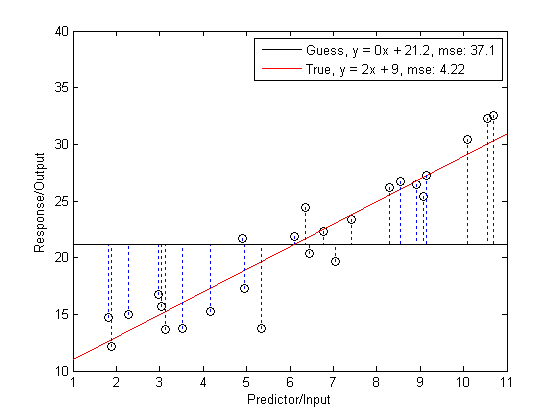
\includegraphics[height=60mm]{g1.png}
\end{figure}
}

\frame[t] {%%%change pic%%%
 \frametitle{Guess \#2}
\begin{figure}
  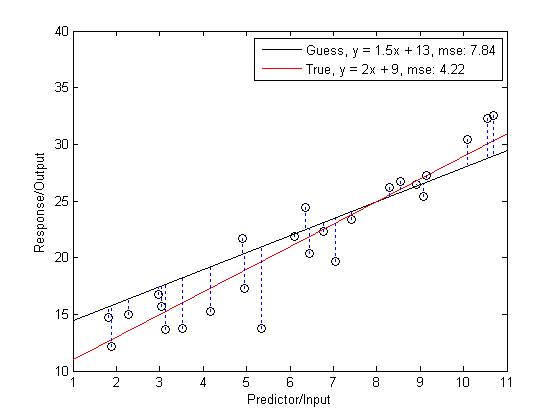
\includegraphics[height=60mm]{g2.png}
\end{figure}
}

\frame[t] {
 \frametitle{Function maximization}
\begin{itemize}
\item Important technique to remember!
\begin{itemize}
\item Take derivative
\item Set result equal to zero and solve
\item Test second derivative at that
point
\end{itemize}
\item Question: does this always give you the maximum?
\item Going further: multiple variables, convex optimization
\end{itemize}
}

\frame[t] {%%%change pic%%%
 \frametitle{Function Maximization}
Find the maximum value of x that satisfies the function $$-x^2 +
ln(x) = a, x>0$$
\begin{figure}
  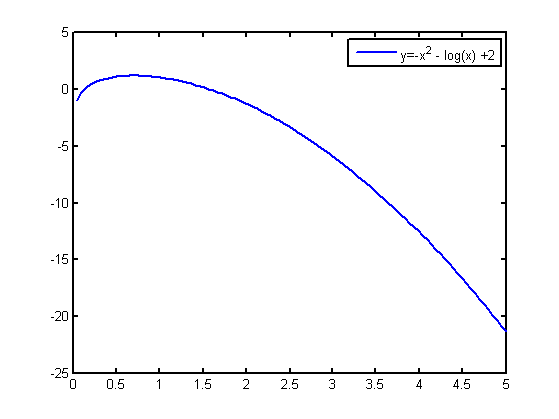
\includegraphics[height=60mm]{fmax.png}
\end{figure} }

\frame[t] {
 \frametitle{Least Squares Max(min)imization}
\begin{itemize}
\item Function to minimize w.r.t. $b_0$ and $ b_1$ -- $b_0$ and $b_1$ are called point estimators of $\beta_0$ and $\beta_1$ respectively
$$Q = \sum_{i=1}^n (Y_i - (b_0 + b_1 X_i))^2$$
\item Minimize this by maximizing -Q

\item Either way, find partials and set both equal to zero
\begin{eqnarray*}
\frac{dQ}{db_0} &=& 0 \\
\frac{dQ}{db_1} &=& 0
\end{eqnarray*}

\end{itemize}
}

\frame[t] {
 \frametitle{Normal Equations}
\begin{itemize}
\item The result of this maximization step are called the normal equations. 
\begin{eqnarray*}
\sum Y_i &=& nb_0 + b_1 \sum X_i \\
\sum X_iY_i &=& b_0 \sum X_i + b_1 \sum X_i^2
\end{eqnarray*}

\item This is a system of two equations and two unknowns.  The solution is given
by$\ldots$

\end{itemize}
}

\frame[t] {
 \frametitle{Solution to Normal Equations}
After a lot of algebra one arrives at
\begin{eqnarray*}
b_1 &=& \frac{\sum(X_i - \bar X)(Y_i - \bar Y)}{\sum(X_i-\bar X)^2} \\
b_0 &=& \bar Y - b_1 \bar X\\
\bar X &=& \frac{\sum X_i}{n} \\
\bar Y&=&\frac{\sum Y_i}{n}
\end{eqnarray*}

}


\end{document}
